\section*{Phụ lục 1: Mã nguồn Python/Qiskit}
\addcontentsline{toc}{section}{Phụ lục 1: Mã nguồn Python/Qiskit}

Toàn bộ mã nguồn Python/Qiskit cho mô phỏng thuật toán Deutsch--Jozsa
được trình bày tại: \url{https://github.com/tdattm/Deutsch-Jozsa.git}

\section*{Phụ lục 2: Các cổng lượng tử và ký hiệu mạch}
\addcontentsline{toc}{section}{Phụ lục 2: Các cổng lượng tử và ký hiệu mạch}
\begin{figure}[H]
    \centering
    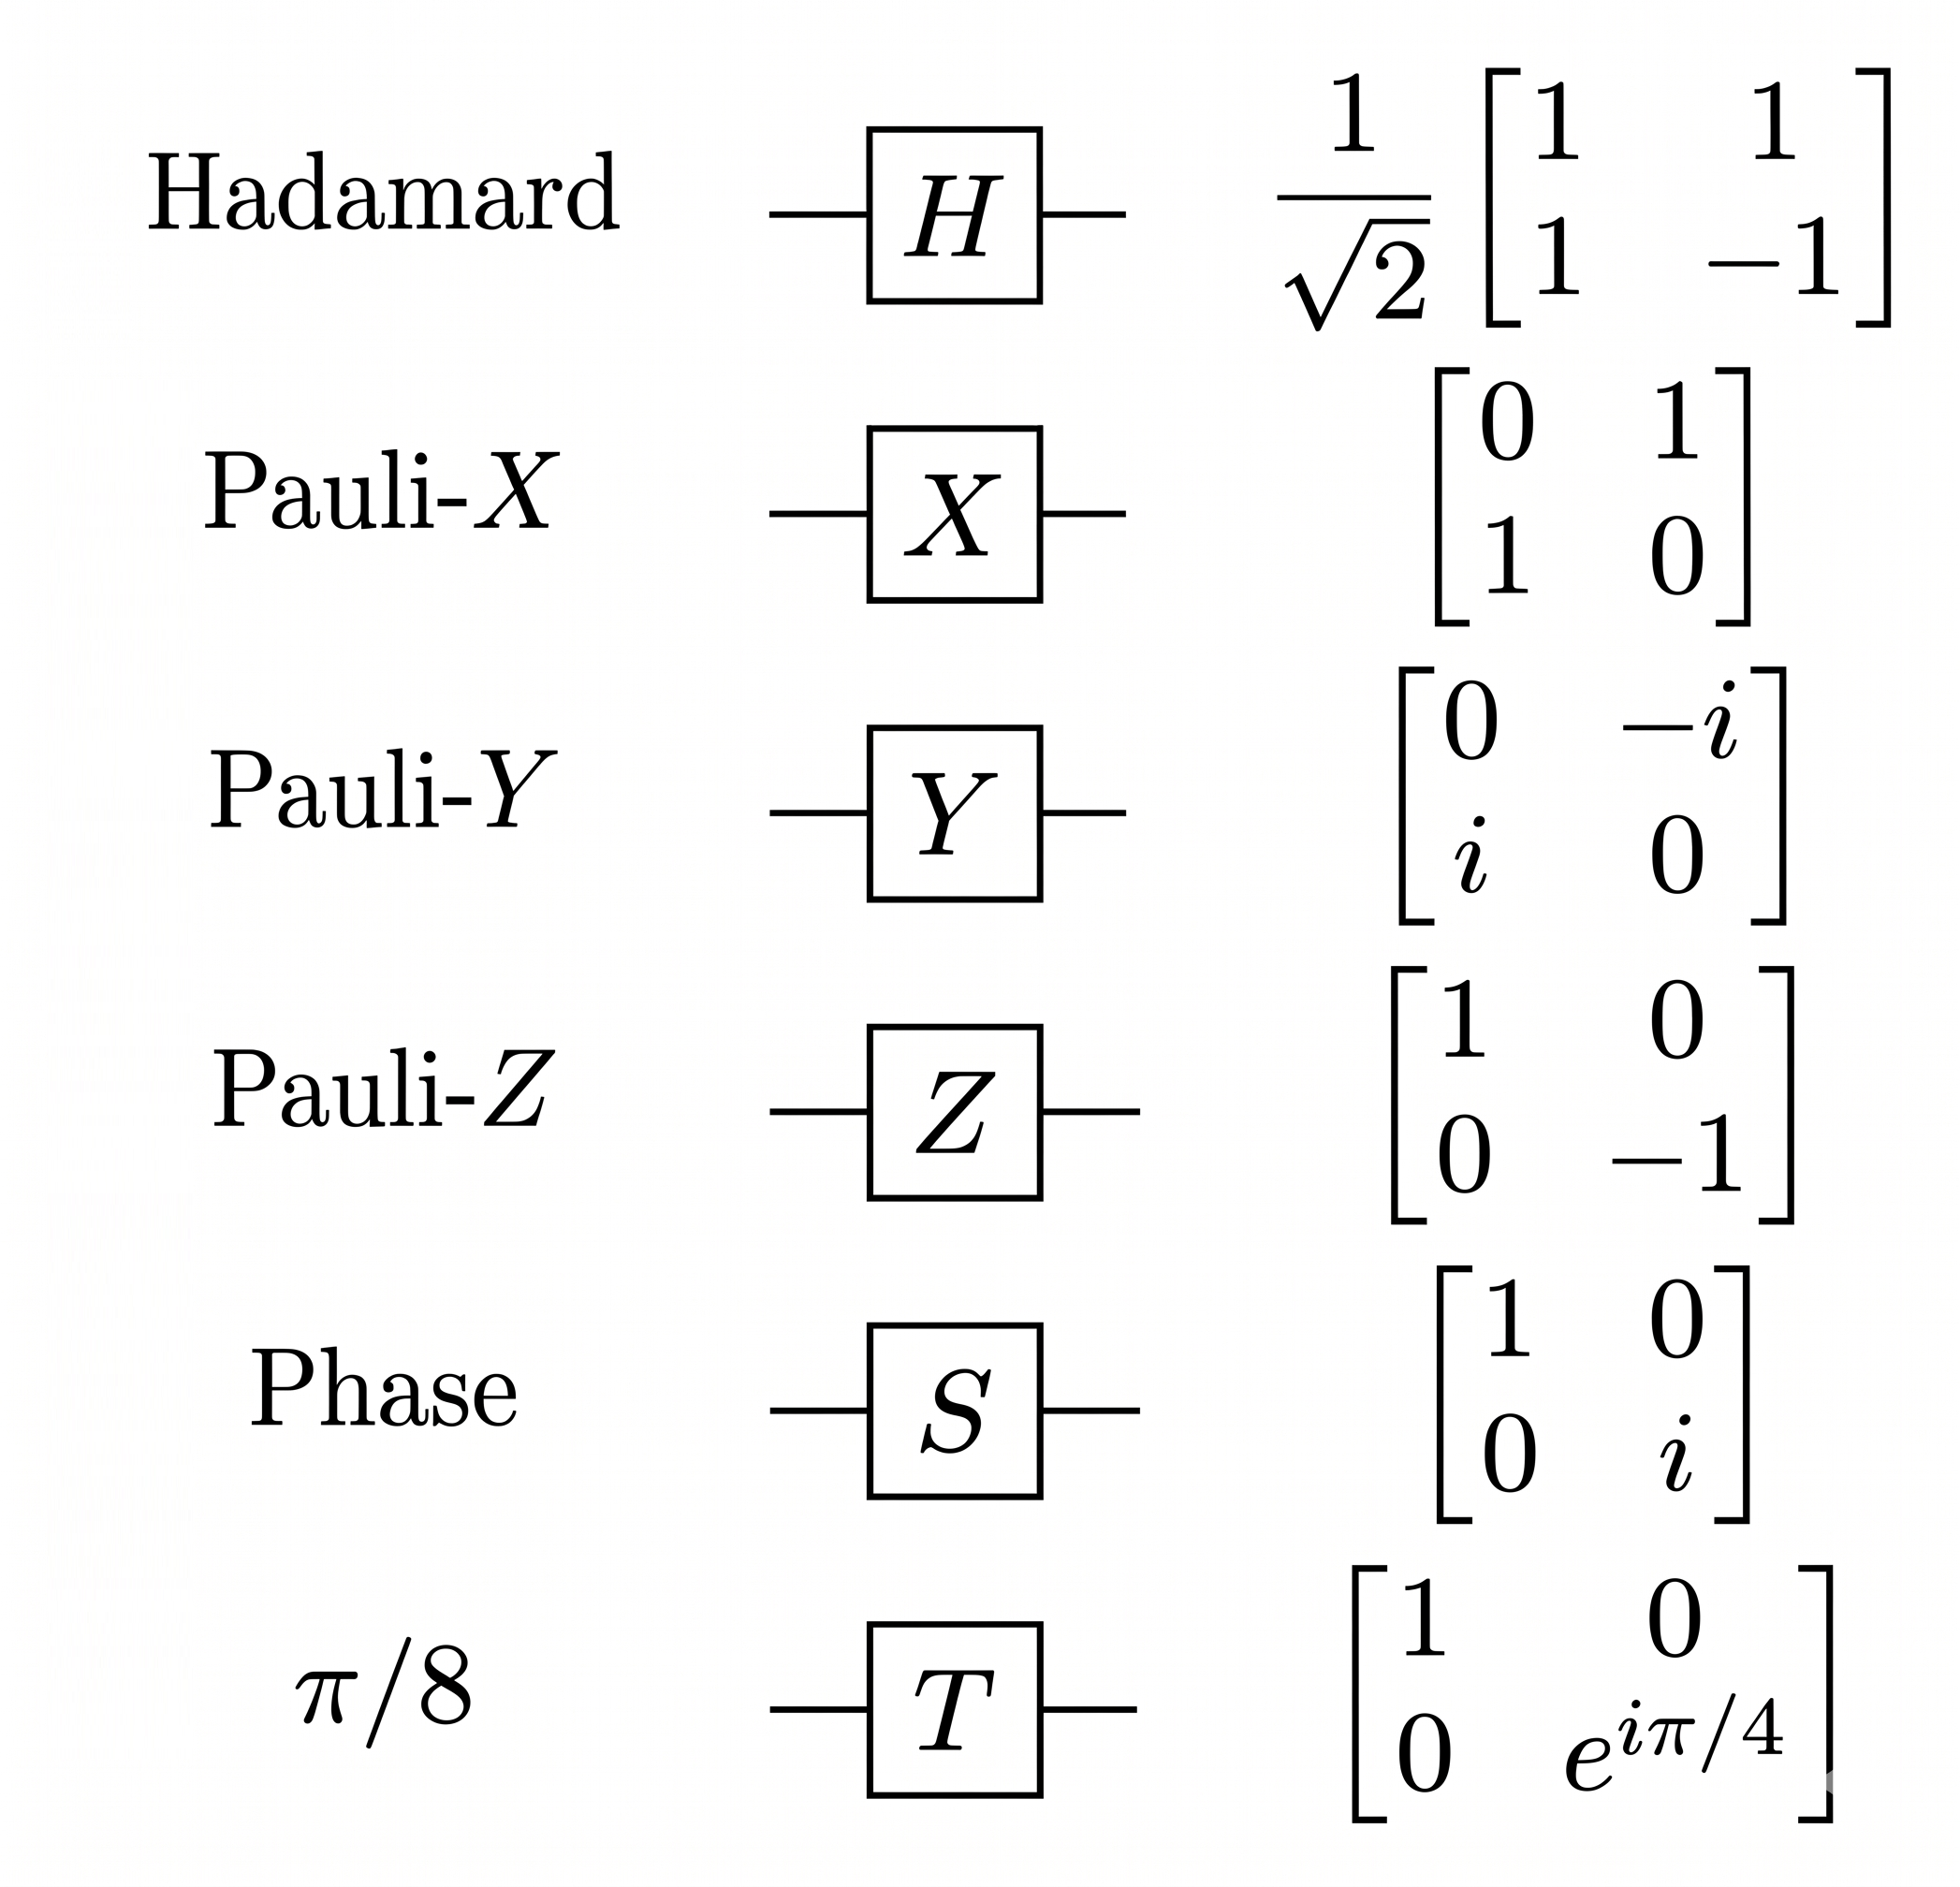
\includegraphics[width=0.7\textwidth]{assets/quantumGates-1.png} 
\end{figure}

\begin{figure}[H]
    \centering
    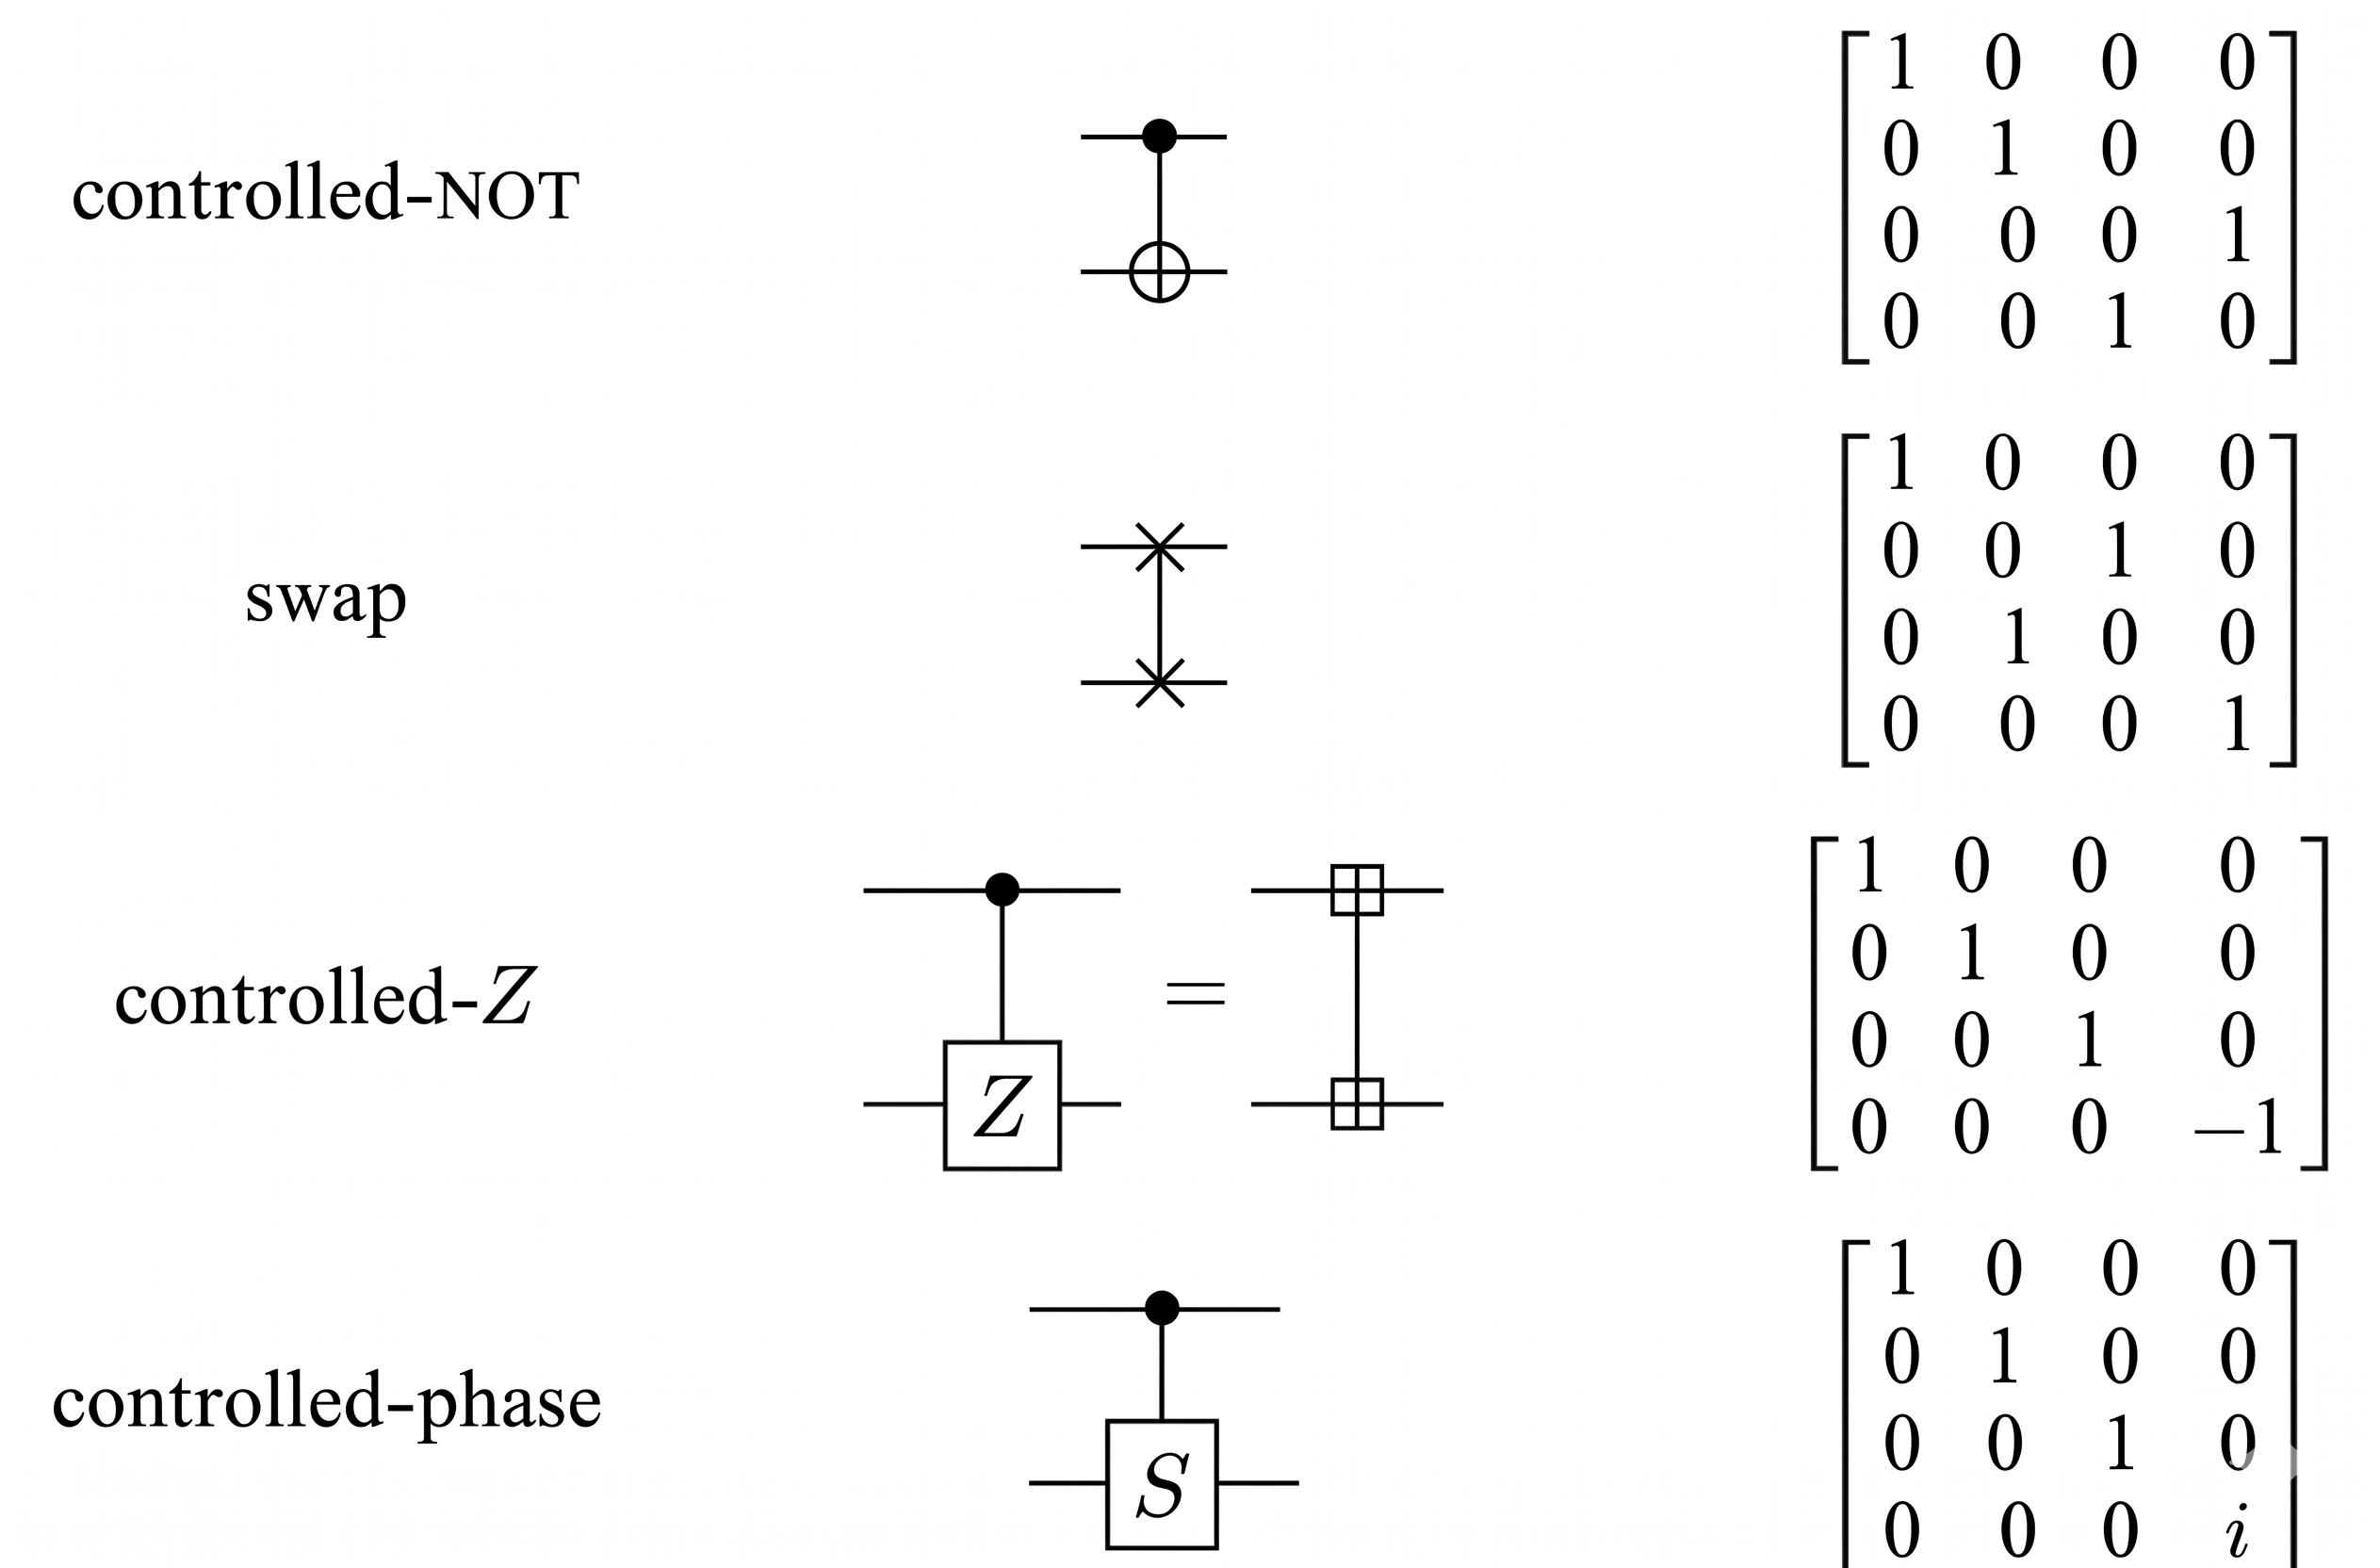
\includegraphics[width=0.9\textwidth]{assets/quantumGates-2.png} 
\end{figure}

\begin{figure}[H]
    \centering
    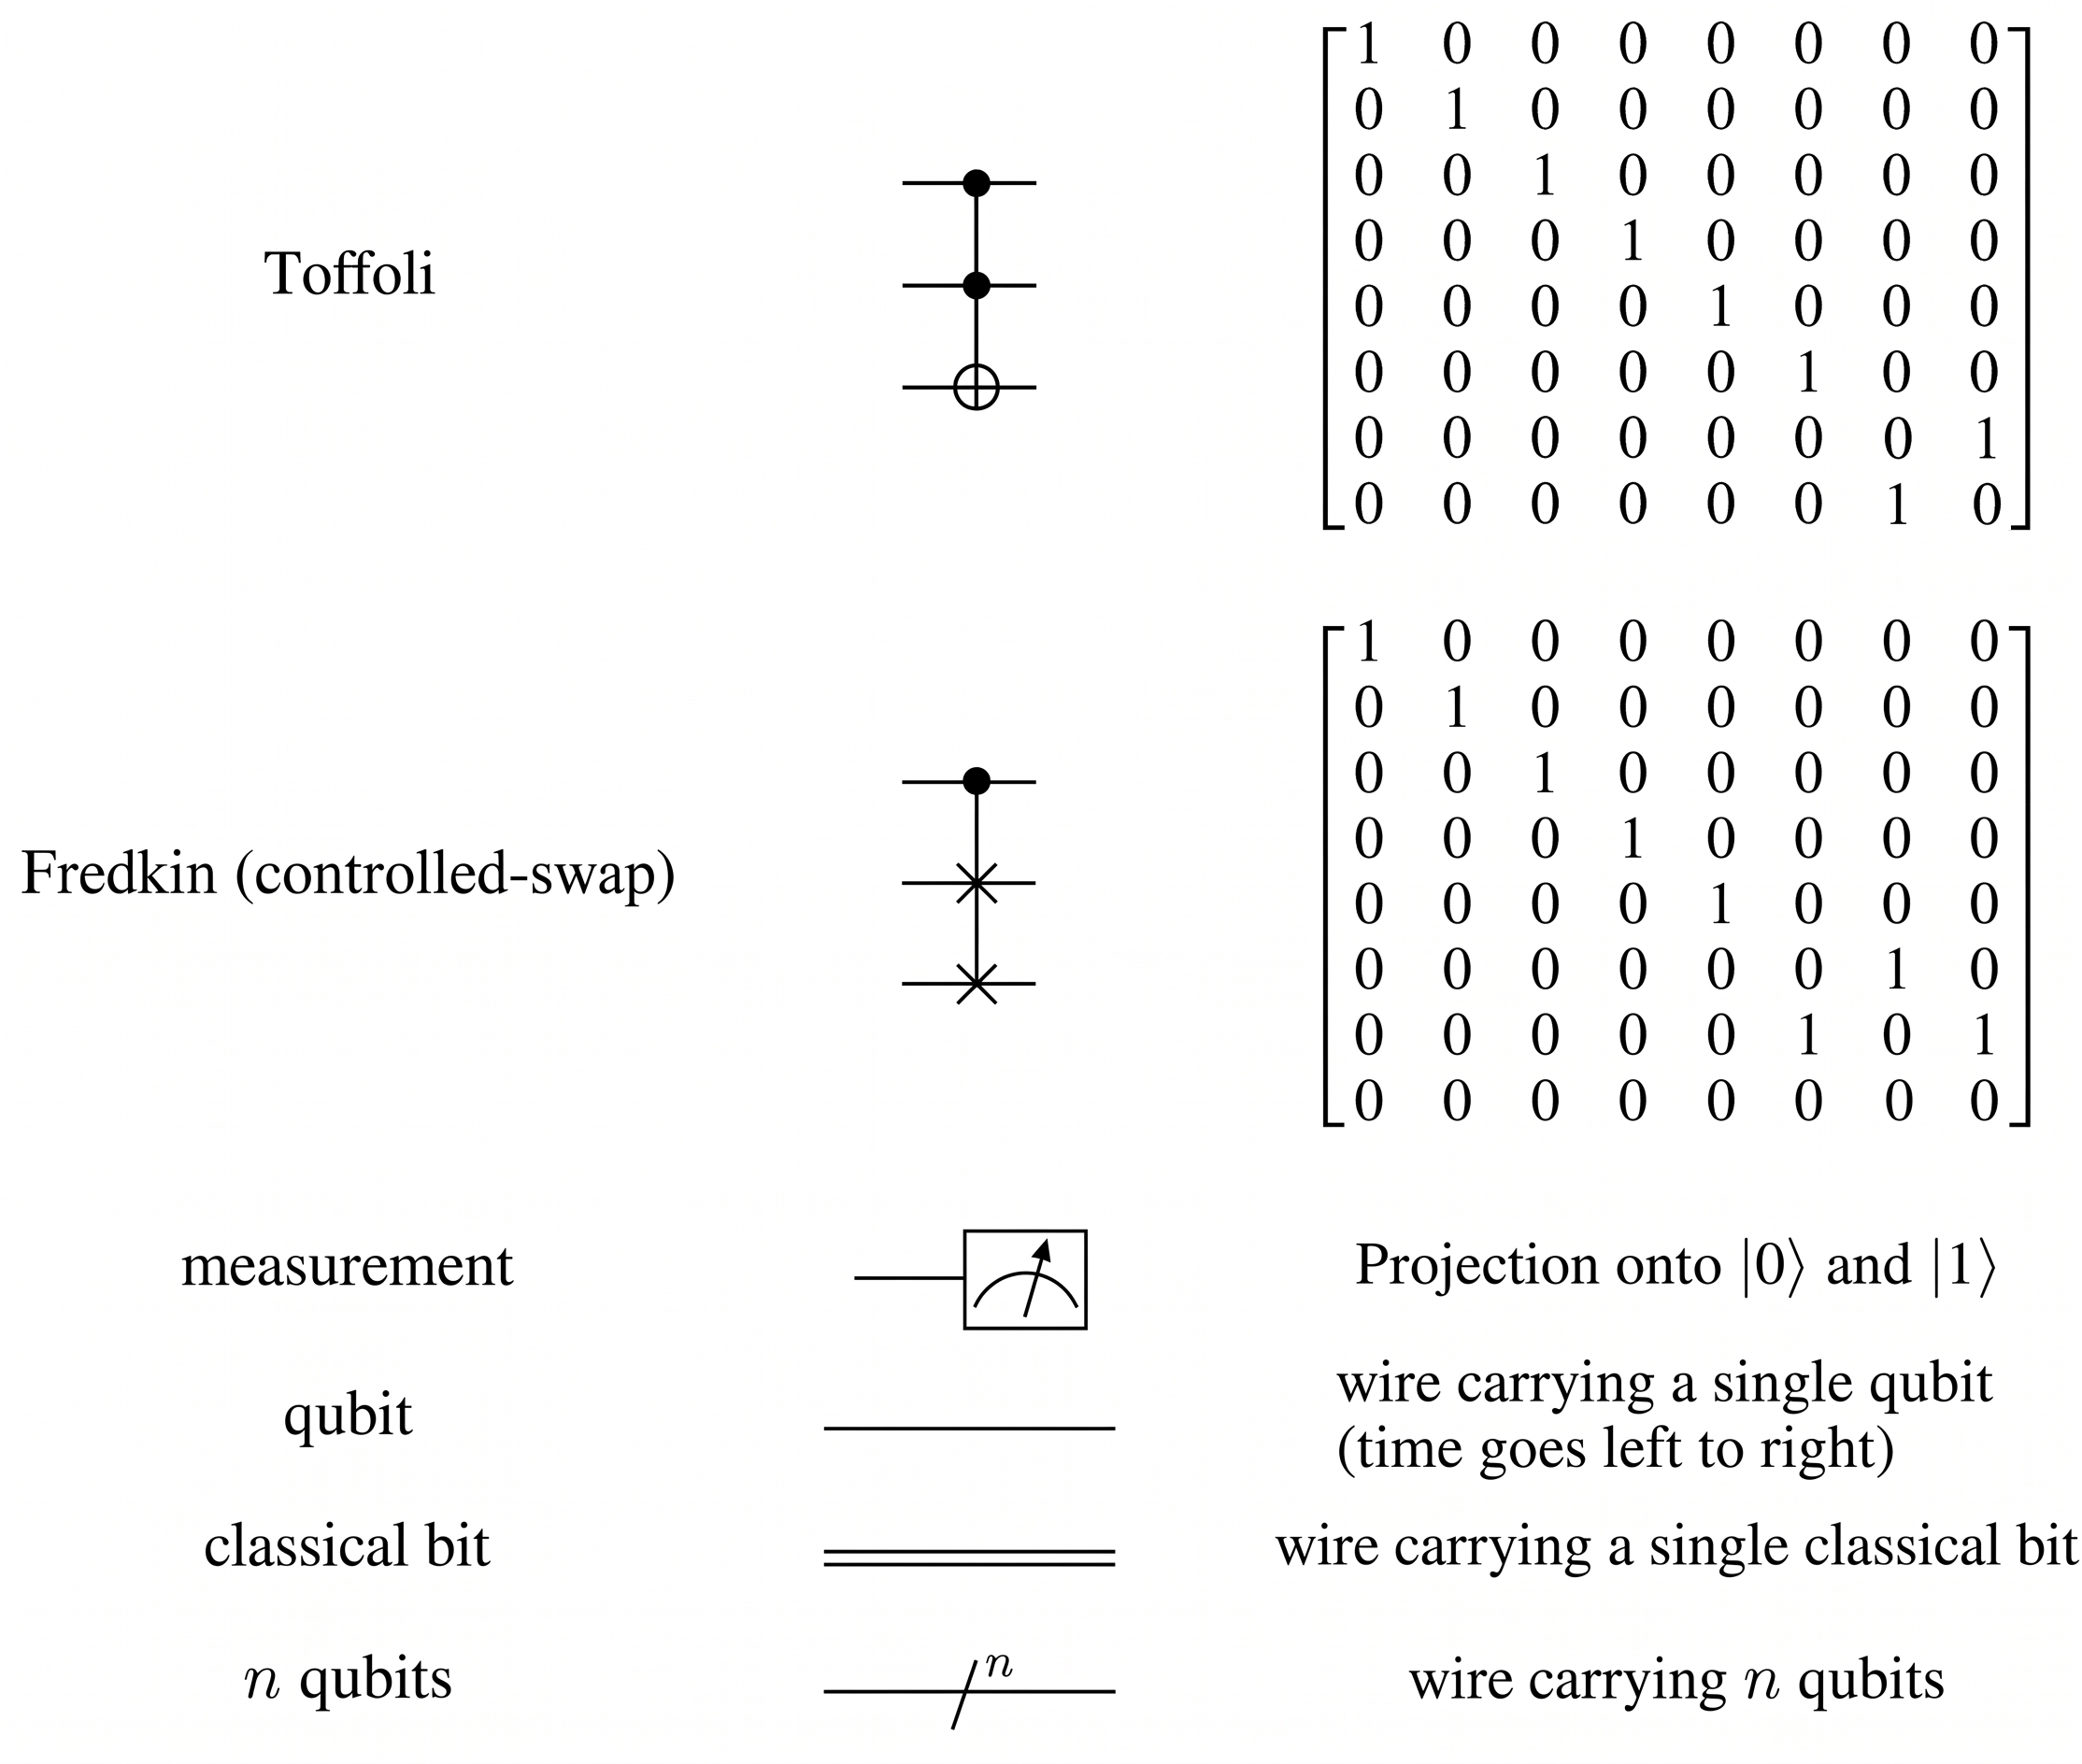
\includegraphics[width=0.9\textwidth]{assets/quantumGates-3.png} 
    \caption{Ký hiệu mạch các cổng lượng tử phổ biến.}
    \vspace{0.2cm}
    \small\textit{Nguồn: \cite{ref5}}
\end{figure}

\section*{Phụ lục 3: Biểu diễn số phức và công thức Euler}
\addcontentsline{toc}{section}{Phụ lục 3: Biểu diễn số phức và công thức Euler}
\label{app:complex}

Phụ lục này tóm tắt cách chuyển đổi một số phức từ dạng đại số sang dạng Euler,
phục vụ cho việc hiểu khái niệm pha toàn cục và pha tương đối trong
mục~\ref{sec:qubit}.

Cho số phức $\alpha = a + bi$ với $a, b \in \mathbb{R}$, trong đó $a$ là phần
thực và $b$ là phần ảo. Số phức này có thể được biểu diễn trực quan như một điểm
(hoặc vectơ) trên mặt phẳng phức, với trục hoành là trục thực và trục tung là
trục ảo.

\begin{figure}[htbp]
    \centering
    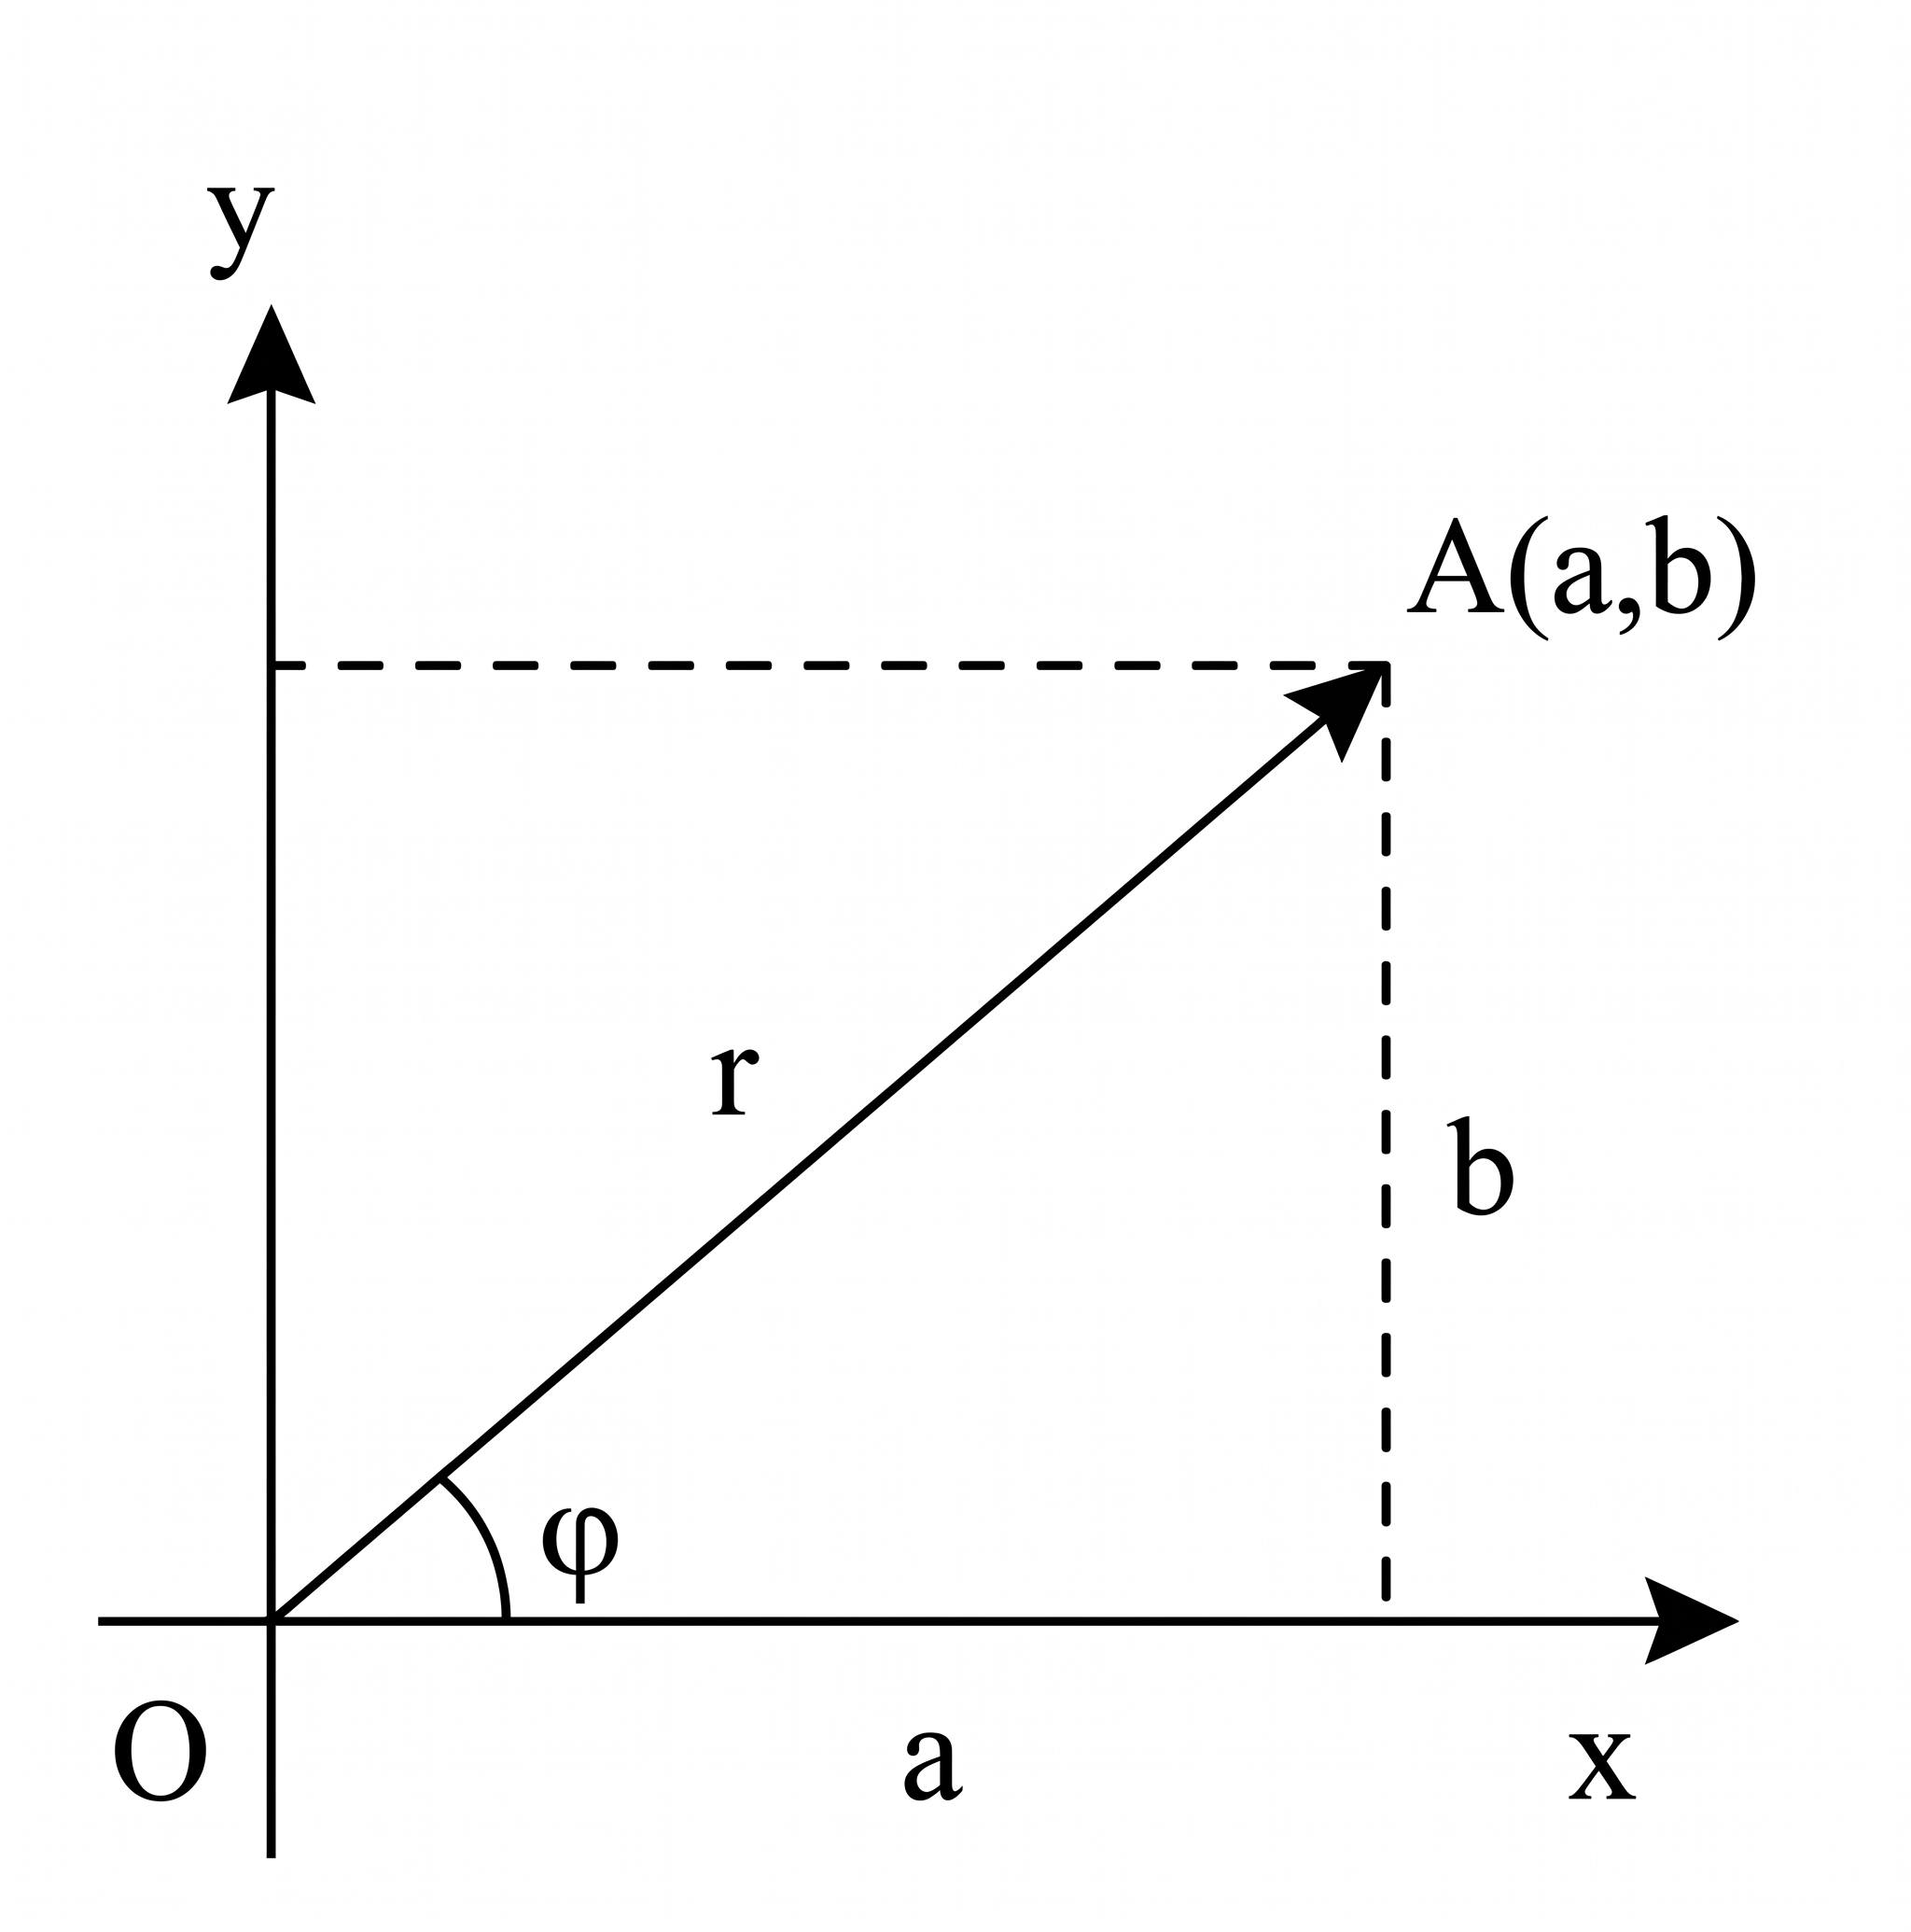
\includegraphics[width=0.5\textwidth]{assets/sophuc.png}
    \caption{Biểu diễn số phức $\alpha = a + bi$ trên mặt phẳng phức.}
    \label{fig:sophuc}
    \vspace{0.2cm}
    \small\textit{Nguồn: Khoa Vật lý, Đại học Sư phạm Tp.HCM.}
\end{figure}

\paragraph{(a) Dạng lượng giác.}
Từ hình học mặt phẳng, vectơ $(a, b)$ có độ dài $r$ và tạo với trục thực một góc
$\theta$, nên các thành phần được biểu diễn qua:
$$a = r\cos\theta, \qquad b = r\sin\theta,$$
trong đó:
$$r = |\alpha| = \sqrt{a^2 + b^2} \quad \text{(môđun)},
\qquad \tan\theta = \frac{b}{a} \quad \text{($\theta$: argument)}.$$
Thay vào $\alpha = a + bi$, ta được \textbf{dạng lượng giác}:
$$\alpha = r(\cos\theta + i\sin\theta).$$

\paragraph{(b) Dạng Euler.}
Công thức Euler khẳng định rằng với mọi $\theta \in \mathbb{R}$:
$$e^{i\theta} = \cos\theta + i\sin\theta.$$
Thay vào dạng lượng giác, số phức $\alpha$ được viết gọn thành
\textbf{dạng Euler}:
\begin{equation}
    \alpha = r\,e^{i\theta}.
    \label{eq:euler}
\end{equation}

% ===============================================================
\section*{Phụ lục 4: Nguồn gốc phương trình tham số hóa mặt cầu Bloch}
\addcontentsline{toc}{section}{Phụ lục 4: Nguồn gốc phương trình tham số hóa mặt cầu Bloch}

Phụ lục này trình bày chi tiết cách dẫn xuất phương trình tham số hóa trạng thái
qubit trên mặt cầu Bloch của phương trình~\eqref{eq:bloch-param} từ dạng tổng quát phương trình~\eqref{eq:qubit}. Nội dung này thuộc vào mục 2.1 của chương 2.

% ---------------------------------------------------------------
\paragraph{(a) Đếm bậc tự do thực}

Trạng thái tổng quát của một qubit là
\[
    |\psi\rangle = \alpha|0\rangle + \beta|1\rangle,
    \quad \alpha, \beta \in \mathbb{C},
\]
trong đó $\alpha$ và $\beta$ mỗi số phức mang hai bậc tự do thực (phần thực và
phần ảo), nên tổng cộng có \emph{bốn} bậc tự do thực. Hai ràng buộc lần lượt
loại bỏ hai trong số đó:

\begin{enumerate}
    \item \textbf{Điều kiện chuẩn hóa} $|\alpha|^2 + |\beta|^2 = 1$ là một
          phương trình thực, loại bỏ một bậc tự do.
    \item \textbf{Pha toàn cục} không có ý nghĩa vật lý: hai trạng thái
          $|\psi\rangle$ và $e^{i\gamma}|\psi\rangle$ cho cùng xác suất đo
          trong mọi cơ sở, nên được đồng nhất về mặt vật lý. Điều này loại
          bỏ thêm một bậc tự do.
\end{enumerate}

Sau hai ràng buộc, còn lại đúng \textbf{hai bậc tự do thực} -- vừa đủ để biểu
diễn bằng hai góc $(\theta, \phi)$ trên mặt cầu đơn vị trong $\mathbb{R}^3$.


% ---------------------------------------------------------------
\paragraph{(b) Tham số hóa modulus bằng góc lượng giác}

Viết $\alpha$ và $\beta$ theo dạng cực:
\[
    \alpha = r_\alpha \, e^{i\varphi_\alpha}, \qquad
    \beta  = r_\beta  \, e^{i\varphi_\beta},
    \quad r_\alpha, r_\beta \geq 0.
\]
Điều kiện chuẩn hóa trở thành $r_\alpha^2 + r_\beta^2 = 1$, có dạng hệ thức
Pythagore. Đặt:
\[
    r_\alpha = \cos\frac{\theta}{2}, \qquad
    r_\beta  = \sin\frac{\theta}{2}, \qquad \theta \in [0, \pi].
\]
Lý do chọn $\frac{\theta}{2}$ thay vì $\theta$: khi $\theta$ chạy từ $0$ đến $\pi$,
góc $\frac{\theta}{2}$ chạy từ $0$ đến $\pi/2$, đảm bảo $\cos(\frac{\theta}{2}) \geq 0$ và
$\sin(\frac{\theta}{2}) \geq 0$, tức $r_\alpha, r_\beta \geq 0$ luôn thỏa mãn mà
không cần ràng buộc thêm. Thay vào trạng thái:
\[
    |\psi\rangle
    = \cos\frac{\theta}{2}\,e^{i\varphi_\alpha}|0\rangle
    + \sin\frac{\theta}{2}\,e^{i\varphi_\beta}|1\rangle.
\]

% ---------------------------------------------------------------
\paragraph{(c) Loại bỏ pha toàn cục}

Nhân toàn bộ $|\psi\rangle$ với $e^{-i\varphi_\alpha}$ -- đây là phép nhân
pha toàn cục, không thay đổi bất kỳ xác suất đo nào:
\[
    |\psi\rangle \;\sim\; e^{-i\varphi_\alpha}|\psi\rangle
    = \cos\frac{\theta}{2}|0\rangle
    + \sin\frac{\theta}{2}\,e^{i(\varphi_\beta - \varphi_\alpha)}|1\rangle.
\]
Đặt $\phi = \varphi_\beta - \varphi_\alpha \in [0, 2\pi)$ là \textbf{pha tương
đối} -- bậc tự do pha duy nhất còn ý nghĩa vật lý. Ta thu được:
\[
    |\psi\rangle = \cos\frac{\theta}{2}|0\rangle
                + e^{i\phi}\sin\frac{\theta}{2}|1\rangle,
\]
đúng với phương trình~\eqref{eq:bloch-param}.